\chapter{A Code Transformations Paradigm for Design Optimization Frameworks}
\label{chap:code_transformations}

This chapter introduces a new paradigm for engineering design optimization frameworks called \textit{code transformations}. Section \ref{sec:definitions} defines the paradigm and introduces the concept of code traceability. Section \ref{sec:aerosandbox} presents AeroSandbox, a reference implementation of this paradigm. Section \ref{sec:benchmarks} benchmarks this framework against existing ones, measured by the technical and non-technical metrics of Figure \ref{fig:birds_eye_view}. Finally, Section \ref{sec:syntax-interface} introduces observations of ideal syntax and interface design for MDO frameworks.

\section{Introduction and Definitions}
\label{sec:definitions}

In recent years, several advanced scientific computing techniques have proliferated that offer fundamentally new capabilities by using non-standard interpretations of numerical code \cite{rackauckas_generalizing_2021}. Examples of these techniques include:

\begin{itemize}[noitemsep]
    \item Automatic differentiation \cite{griewank_automatic_1988}, a technique that allows efficient and accurate evaluation of a function's gradient at runtime
    \item Automatic sparsity detection \cite{gebremedhin_efficient_2009}, a technique that identifies which of a function's outputs may be affected by each input
    \item Automatic problem transformations (in the context of numerical optimization), including techniques such as:
    \begin{itemize}[noitemsep]
        \item Problem scaling \cite{nocedal_numerical_2006}, to improve the conditioning of Hessians and linear sub-problems
%        \item Log-transformations of variables, constraints, and objectives (similar to geometric programming) \cite{kirschen, agrawal_disciplined_2019}, which can improve convexity or eliminate nonlinearities
        \item Redundant constraint elimination
    \end{itemize}
    \item Common subexpression elimination \cite{casadi}, where repeated calculations are automatically identified and rewritten for faster speed via pre-computation
    \item Backend-agnostic programming, which can enable hardware accelerators (e.g., GPUs), different math library backends, just-in-time (JIT) compilation, and automatic vectorization \& parallelization \cite{jax}
\end{itemize}

In this work, we collectively call this set of computational techniques \emph{code transformations}. Formally defined, a code transformation is any operator\footnote{i.e., a higher-order function} that a) intercepts some representation of the user's original code at runtime, b) automatically applies some improvement based on analysis of the code itself, and c) returns this improved function to be executed in-place of the original.
%Code transformations are essentially the union of two related existing computer science concepts: compiler optimizations and scientific machine learning.

This definition is similar to that of a ``compiler optimization'' in computer science, though a distinction can be drawn in the implied level of code abstraction where the improvement is applied. Compiler optimizations typically refer to lower-level improvements at the level of source code static analysis or a language-level syntax tree (e.g., dead-code elimination, loop fusion, and static type inference and specialization). By contrast, code transformations broaden this to also include improvements at the higher level of computational graphs dynamically constructed within domain-specific modeling languages, or at the level of a data structure describing a complete numerical method (e.g., an optimization problem formulation).

Another useful point of comparison for this code transformations definition is ``scientific machine learning'' (SciML), which is a term that has become increasingly popular to describe several of these higher-level transformations \cite{ma_modelingtoolkit_2021, hu_taichi_2018, lavin_simulation_2022}. In particular, this term has been applied to end-to-end automatic differentiation of physical simulators, especially in cases where it is then used for machine learning applications such as parameter estimation, surrogate modeling, or scientific hypothesis testing via probabilistic programming. SciML methods can be seen as a subset of code transformation techniques that emphasize differentiability and compatibility with machine learning frameworks, and implementations often make various engineering tradeoffs that favor this goal \cite{rackauckas_engineering_2021}. Therefore, an informal definition of code transformations is that it is a union of both compiler optimizations and scientific machine learning.

%as well as the composability of such transformations through their expression as higher-order functions \cite{jax}. A beneficial consequence of this dynamic, composability-first point of view has been the growth of modeling languages \cite{_modelica_2023, ma_modelingtoolkit_2021, _simulink_2020, fourer_ampl_1989} and domain-specific languages for machine learning \cite{pytorch, hu_taichi_2018}, which can offer reduced barrier to entry.

% separates declarative and imperative code; HTML/CSS,
% undersells impact—not just ml

\subsection{Code Traceability}
\label{sec:traceability}

The main benefit of generalizing these techniques under a ``code transformations'' abstraction is to highlight that all of these advanced techniques essentially impose the same shared requirement on numerical code: a property we refer to as code \emph{traceability}. Here, a piece of numerical code is defined as ``traceable'' if we can construct and directly inspect some functional representation (often, a computational graph) of this code at runtime.

There are several possible ways to construct and access these functional representations in a way that meets this definition, but the most common method (and the one used throughout this work) is aptly called \emph{tracing} in the machine learning literature\footnote{Tracing is not the only means by which code transformations can be performed—one example alternative is direct source code transformation, which can be seen in frameworks like Tapenade \cite{tapenade}. However, tracing-like strategies are by far the most common in modern, syntactically-rich languages; comprehensive discussion of the tradeoffs and motivations for this are given by Maclaurin \cite{maclaurin_modeling_2016}.} \cite{jax, frostig_compiling_2018, baydin_automatic_2018}. This process involves taking functional numerical code, and, rather than evaluating it with standard numerical inputs, instead passing in a ``tracer'': a symbolic-like dummy data type that records operations performed on it\footnote{In some frameworks, the tracer is used only for graph construction (e.g., JAX's \texttt{Tracer} \cite{jax}). In others, the same object serves an additional purpose during numerical evaluation, where it works as a concrete numerical data type (e.g., PyTorch's \texttt{Tensor} \cite{paszke_pytorch_2019}).}. The output of the code then includes a recorded computational graph representing the code execution path (the ``trace'' or ``tape'' \cite{paszke_pytorch_2019}), which can then be manipulated and transformed to enable the advanced techniques listed above.

For this tracing process to work, all mathematical functions used within this numerical code must be able to accept and return these tracer objects\footnote{Another observation is that this tracing process is generally easier to implement in languages with dynamic typing or multiple dispatch, as these languages make it easier to switch between traditional and tracer data types in numerical code.}. In practice, this often means that traceable code must be written with a specialized numerical framework that accepts that tracer type—we must be able to intercept math library calls in order to properly handle tracers. This also implies that traceability is a property that is defined with respect to a specific numerical framework, rather than a universal property of the code itself.

This concept of traceability allows us to intuitively predict which operations are likely to ``break the trace'' and render the target code incompatible with code transformations. For example, explicit type casting often causes problems, since a tracer variable may be coerced into a concrete numerical type, resulting in a lost computational graph. Likewise, any interfaces between programming languages (e.g., a Python function calling a C function) will usually break the trace, as type information is lost across the language boundary. This insight can be used to guide the design of numerical code to be more traceable, and hence more amenable to code transformations.

Traceability is also the reason why it can be challenging to add many of these advanced techniques (e.g., end-to-end problem-level automatic differentiation) into an MDO framework unless it was designed to support these from the start. For example, often standard MDO disciplinary interfaces only allow for concrete numerical data types; so, while individual analyses may be traceable, tracing the full optimization problem end-to-end is usually not possible unless the framework accommodates this. This inherently limits the kinds of problem accelerations that can be applied. As a more concrete example of this, one may find themselves able to use AD to find the partials of a single analysis, but directly computing the constraint Jacobian of the full MDO problem may not be possible\footnote{Instead, the framework needs to stitch these partials together. This becomes particularly messy if tracers cannot be end-to-end propagated through analyses that project from low- to high- to low-dimensionality spaces, like from a design space (low-dim) to a mesh space (high-dim) to an output space (low-dim). Here, the user needs to manually implement some kind of forward-over-reverse AD gradient stitching, rather than letting the framework handle it end-to-end. This may be acceptable for one or two disciplines, but for problems with dozens of interacting submodels it becomes overly burdensome for the user. It also splits the computational graph at these large intermediate data structures, which can cost speed.}. This is a key motivation for the development of a new paradigm for MDO frameworks that considers traceability from the start, as opposed to simply adding on these advanced scientific computing techniques to existing paradigms.

\subsection{Implications for Engineering Design}

The main goal of this chapter is to introduce this idea of code transformations (via traceable code) as a possible computational paradigm on top of which an MDO framework can be built. This work deliberately aims to broaden the focus of framework design towards traceability, rather than towards any one specific transformation technique (e.g., automatic differentiation). By finding this common thread, we enable a much more general set of computational techniques to be applied, and this approach remains more scalable as new transformation techniques are developed.

If these code transformation techniques can be applied to engineering design optimization, they could offer significant runtime speed improvements over the black-box optimization methods that form the vast majority of industry use today \cite{martins_engineering_2021, lavin_simulation_2022}. As shown later in this chapter, these achievable speeds are comparable to those of state-of-the-art optimization methods in academia, such as disciplined optimization methods\footnote{such as geometric programming and disciplined convex programming} \cite{grant_disciplined_2006, gpkit, boyd_convex_2004, agrawal_disciplined_2019} and gradient-based methods using user-provided analytic gradients\footnote{sometimes referred to as ``adjoint methods'' in reference to a common method for manually deriving these gradients for more-complex analyses} \cite{gray_openmdao_2019, kenway_effective_2019, innes_don_2019}.

A crucial advantage of code transformation over many state-of-the-art methods is that they can be applied mostly \textit{automatically} -- most of the benefits of these advanced techniques can be gained without requiring any additional effort (or mathematical expertise) from the user. This ease-of-use is critical for practicality -- Grant notes that many existing paradigms are hamstrung by a ``expertise barrier'' \cite{grant_disciplined_2006}, which inhibits industry adoption. To assess this further, Table \ref{tab:paradigm_comparison} compares code transformations to existing MDO paradigms across three key practical metrics. These metrics are derived from the high-level view of the user frictions in engineering design optimization, as given in Figure \ref{fig:birds_eye_view}. Considerations and further discussion of these tradeoffs are given in Appendix \ref{chap:paradigm_comparison}.

\begin{table}[H]

    \newcolumntype{M}{>{\raggedright\arraybackslash}m{0.23\textwidth}}
    \newcolumntype{E}{>{\raggedright\arraybackslash}m{0.19\textwidth}}
    \newcolumntype{I}{>{\centering\arraybackslash}m{0.21\textwidth}}
    \newcolumntype{S}{>{\centering\arraybackslash}m{0.21\textwidth}}
    \newcolumntype{Q}{>{\centering\arraybackslash}m{0.16\textwidth}}

    \definecolor{q1}{HTML}{BA3434}
    \definecolor{q2}{HTML}{458505}
    \definecolor{q3}{HTML}{068383}
    \definecolor{q4}{HTML}{0C6CFD}

    \newcommand{\bad}{\textcolor{q1}{\large\textbf{Limited}}}
    \newcommand{\good}{\textcolor{q2}{\large\textbf{Good}}}
    \newcommand{\great}{\textcolor{q3}{\large\textbf{Great}}}
    \newcommand{\best}{\textcolor{q4}{\large\textbf{Best}}}

    \centering
    \caption{A subjective comparison of tradeoffs between existing MDO framework paradigms and the proposed \textit{code transformation} paradigm. The industrial state-of-the-art is largely de facto \textit{black-box optimization}. The academic state-of-the-art has two major branches: \textit{gradient-based methods with analytical gradients}, and \textit{disciplined optimization methods}. More detailed discussion of these assessments, including definitions and reasoning, is given in Appendix \ref{chap:paradigm_comparison}.}
    \label{tab:paradigm_comparison}

    \begin{adjustbox}{width=\textwidth}
        \setstretch{1.25}
        \begin{tabular}{M E I S Q}
            \toprule
            \textbf{MDO Framework Paradigm}                 & \textbf{Example Frameworks and Tools}                                                                                                                                                                                                       & \textbf{Ease of \mbox{Implementation}}\ (sketchpad-to-code) & \textbf{Runtime Speed and Scalability}\ (code-to-result) & \textbf{Modeling Flexibility} \\ \toprule
            \textbf{Black-box Optimization}                 & SUAVE \cite{SUAVE2017}, OpenMDAO$^*$ \cite{gray_openmdao_2019}, TASOPT \cite{drela_tasopt_2010}, PASS \cite{antoine_framework_2005}, FAST \cite{fast_ga_code}, FLOPS \cite{flops}, FBHALE \cite{fbhale}, \textbf{almost all industry codes} & \great & \bad & \best \\ \midrule
            \textbf{Gradient-based with Analytic Gradients} & MACH-Aero \cite{he_aerodynamic_2018}, OpenMDAO$^*$ \cite{gray_openmdao_2019}, OpenConcept \cite{brelje_multidisciplinary_2021} & \bad & \best & \great \\ \midrule
            \textbf{Disciplined Optimization}               & GPkit \cite{gpkit}, other convex methods \cite{karcher_method_2023, boyd_convex_2004, grant_disciplined_2006}, AMPL \cite{fourer_ampl_1989} & \good & \good & \bad \\ \midrule
            \textbf{Code \mbox{Transformations}}            & AeroSandbox$^\dag$ \cite{sharpe_aerosandbox_2021}, JAX$^\ddag$ \cite{jax}, ModelingToolkit.jl$^\ddag$ \cite{ma_modelingtoolkit_2021} & \good & \great & \good \\
            \bottomrule

            \multicolumn{5}{p{1\textwidth}}{$^*$ Can use either paradigm, depending on user's implementation} \\
            \multicolumn{5}{p{1\textwidth}}{$^\dag$ Introduced as part of the present work} \\
            \multicolumn{5}{p{1\textwidth}}{$^\ddag$ These are computational tools to facilitate code transformations, rather than design optimization frameworks}
        \end{tabular}
    \end{adjustbox}

\end{table}

In short, the main claim this chapter aims to demonstrate is that a code transformations paradigm yields a favorable compromise between all three tradeoffs: it achieves computational speeds similar to the latest academic methods, retains a learning curve comparable to methods already accepted by industry today, and does not impose overly-burdensome mathematical restrictions. If this hypothesis is validated, it leads to a compelling value proposition: if we can develop new methods for industry engineers to easily write traceable design code, then we can give them access to a host of advanced scientific computing techniques and help shrink the academia-industry MDO gap described in Chapter \ref{chap:literature}.

Accordingly, the contribution of this chapter is twofold. First, this chapter will conceptually introduce code transformations as a new paradigm for engineering MDO frameworks. Secondly, the thesis will demonstrate strategies that allow traceability of engineering design code with acceptably low user effort, enabling the use of code transformations in practice.


%Therefore, for the purposes of this work, \textit{traceability} is effectively synonymous with code transformability.


%A key observation is that many of these diverse techniques share similar principles. First, all of these techniques are operations that both act on and return executable code functions, and hence can be mathematically characterized as \emph{higher-order functions}.

% The value proposition of this paradigm is this: if we can reduce user frictions to write traceable code, we can achieve large gains in
%The goal, then, is to enable end users to write traceable code with minimal effort—if this can

%, where numerical code is written in a declarative style that separates numerics from execution. This includes
% Tradition ``compiler optimizations'' -> we look at them as a framework paradigm


\section{AeroSandbox: A Proof-of-Concept Framework Implementation}
\label{sec:aerosandbox}

To research the feasibility, opportunities, and limitations of a code transformations paradigm for engineering design optimization in greater detail, we have developed an experimental MDO framework called \emph{AeroSandbox}. AeroSandbox is implemented as a Python-based framework aimed primarily at supporting conceptual-level engineering design. As a design \emph{framework} (analogous to OpenMDAO \cite{gray_openmdao_2019} or GPkit \cite{gpkit}), AeroSandbox is a library that provides underlying utilities for formulating and solving general design problems -- this is contrasted against a design \emph{tool} that specializes in supporting a targeted design application (e.g., TASOPT \cite{drela_tasopt_2010}). The code is made publicly available under the open-source MIT license with the goal of gathering as much practical user feedback as possible; further access details are given in Section \ref{sec:asb-reproducibility}.

\subsection{Graph Construction and Optimization}

Fundamentally, AeroSandbox is a tool for building and transforming large computational graphs, and indeed these graphs can be directly inspected both computationally and visually, as Figure \ref{fig:computational-graph-aerosandbox} demonstrates. AeroSandbox uses its own specialized numerics module to intercept and trace user code, and it can interface with tracer-like objects from either the CasADi \cite{casadi} or JAX\footnote{Experimentally available via the \texttt{jaxify} branch of the AeroSandbox GitHub repository, linked in Section \ref{sec:asb-reproducibility}.} \cite{jax} libraries to produce a computational graph compatible with these respective libraries. Coverage is provided for a wide range of mathematical functions, including most of the popular NumPy library \cite{harris_array_2020} and key parts of the SciPy library \cite{scipy}.

\begin{figure}[h]
    \centering
    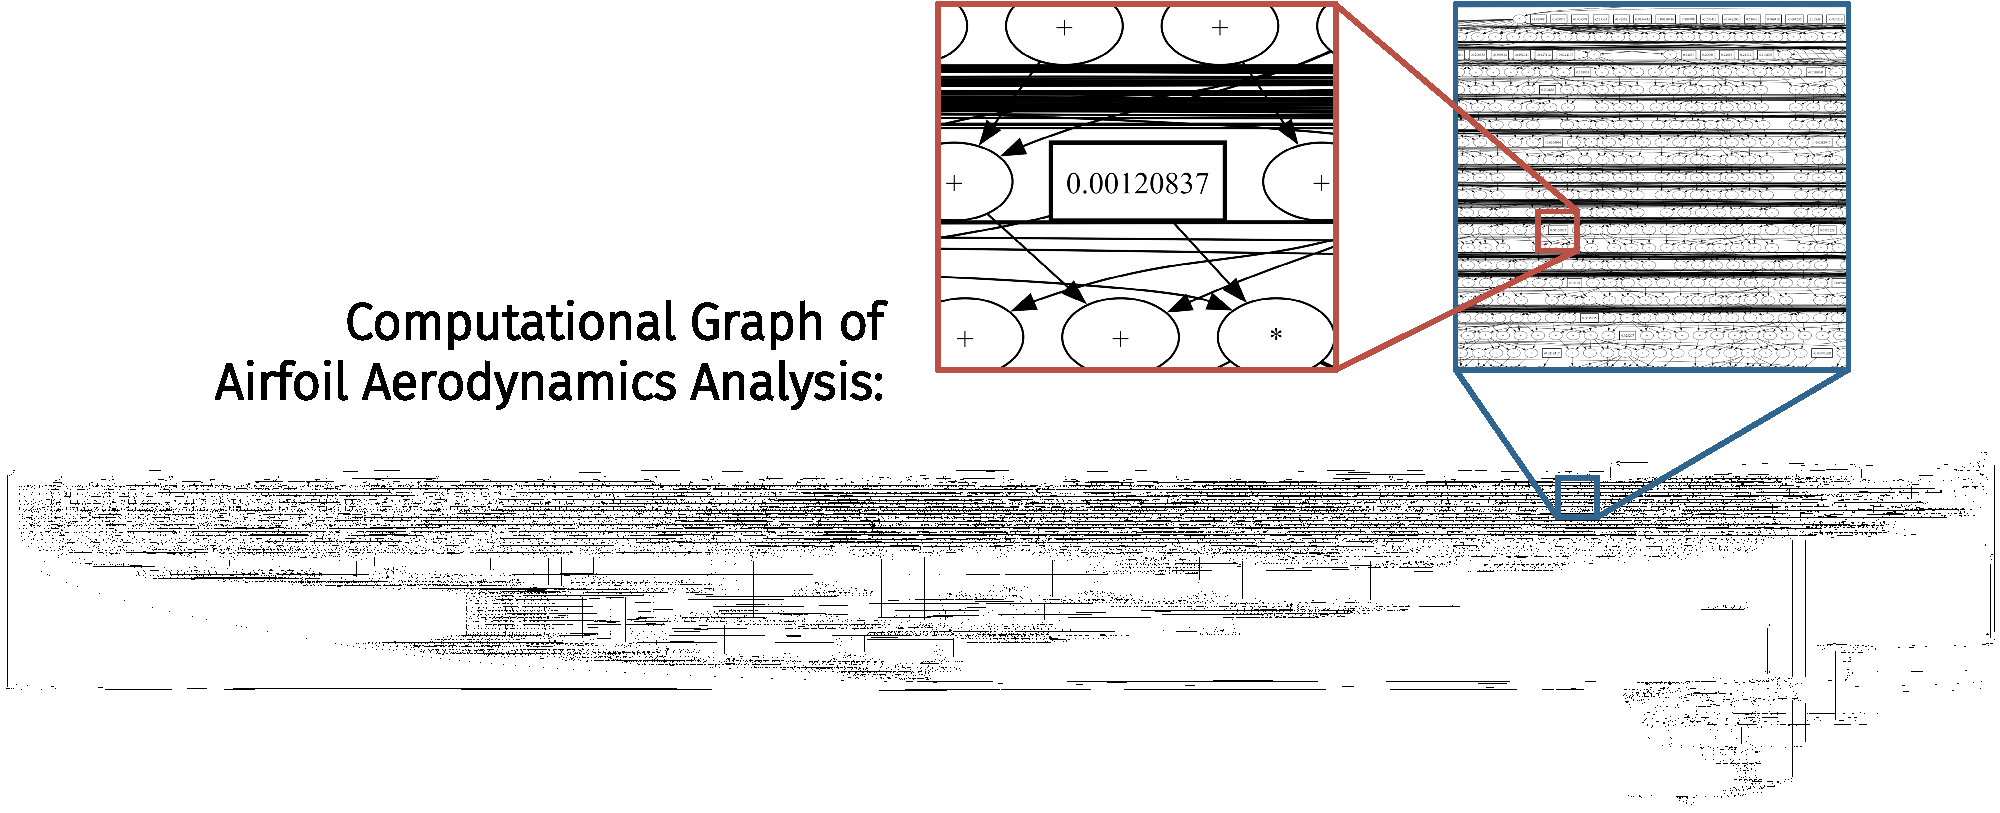
\includegraphics[width=\textwidth]{../figures/large_computational_graph-crop.pdf}
    \caption{An example computational graph, as constructed by AeroSandbox at runtime. Zoomed-in view allows visualization of the scale of such graphs, which can grow to millions of nodes and edges for problems of practical interest. The analysis depicted here is an aerodynamics analysis of an airfoil at a given flow condition, using NeuralFoil (described further in Chapter \ref{chap:physics-informed-ml}). Elements of the analysis that are not functions of design variables are pre-computed and collapsed into a single node in the computational graph, so the exact runtime graph will depend on the user-specified optimization problem formulation.}
    \label{fig:computational-graph-aerosandbox}
\end{figure}

During graph construction, code variables that the user specifies as optimization variables are assigned tracers and included as input nodes to the computational graph. Because this happens at runtime on an as-needed basis, those parts of the computation that are not functions of optimization variables are evaluated as standard numerical functions. This essentially allows static parts of the optimization problem (e.g., constants, parameters, or frozen variables; and any analyses that are a pure function of these) to be evaluated once and then be reused across multiple function evaluations, which can significantly reduce computational overhead.

While constructing this graph, AeroSandbox deliberately makes certain framework-level decisions which are tradeoffs that tend to work well in engineering design optimization, as contrasted with other possible applications like machine learning \cite{rackauckas_engineering_2021}. An example of one such choice is the decision to use static computational graphs, where the graph is constructed once during problem specification, rather than repeatedly at each function evaluation during optimization\footnote{Behavior analogous to this latter approach is seen in PyTorch, for example, where evaluation and tracing happen simultaneously.}. This static approach results in a reduced computational overhead per-function, which is important as engineering analysis tends to involve deep, scalar-heavy\footnote{Relative to traditional machine learning, which tends to focus more on large kernel operations (e.g., matrix multiplication and other einsum-like functions) that perform much more computational ``work'' per call.} computational graphs. This also makes it more worthwhile to apply global transformations (e.g., common subexpression elimination) to the graph, since the overhead of this is only incurred once. On the other hand, this same decision inherently prohibits value-dependent language-level control flow from being recorded in the graph, which creates challenges in other cases (e.g., adaptive-step numerical integrators). Tradeoffs such as this are made at every step of the framework architecture, from graph construction to code transformation heuristics to optimizer strategies; often there are no unconditionally correct choices, and the end result is a framework that makes numerical choices favoring engineering design cases.

Once the graph is constructed, various user-specified inputs and outputs are connected to form a data structure representing a numerical optimization problem. With this information, code transformations can be applied. Most transformations, like automatic differentiation, automated sparsity detection, and problem scaling, are performed automatically and transparently to the user. Here, sensible default heuristics tuned on engineering design optimization problems are used. For example, the framework will automatically choose between forward-mode and reverse-mode automatic differentiation for the constraint Jacobian based on its dimensionality after coloring and compression. Likewise, problem scaling is applied on variables and constraints with a heuristic based on the user-provided initial guess, any bounds constraints, and the constraint Jacobian at the initial guess.

After appropriate code transformations are applied, the transformed problem is then solved using a numerical optimization backend. By default, this backend sends the solve to IPOPT \cite{wachter_implementation_2006}, a second-order gradient-based optimization algorithm that performs favorably in large-scale engineering design optimization \cite{lyu_benchmarking_2014}. Another benefit of IPOPT is that constraints are handled by a primal-dual interior point algorithm, which allows constraint sensitivity information to be obtained naturally as part of the solve. This core mathematical framework architecture, tradeoffs, and heuristics are discussed in further detail in prior work by Sharpe \cite{sharpe_aerosandbox_2021}.

It should be emphasized that this core design optimization framework is intended to be broadly applicable to many kinds of large-scale engineering systems, and is not aerospace-specific. However, on top of this application-agnostic numerical framework, many optional aircraft-design-specific tools and physics modules are included, which make the framework especially well-suited to support these applications. These specialized tools are the focus of Chapter \ref{chap:physics}, though an overview of how these tools fit into the broader framework is given in Figure \ref{fig:asb-diagram}.

\begin{figure}[h]
    \centering
    \providecommand\ntxt{}
\renewcommand{\ntxt}[2]{
    \textbf{#1}\\#2
}

\tikzstyle{int} = [
thick,
rectangle, rounded corners, minimum height=2em,
draw=c1,  fill=c1!20,
text width=11em, text centered,
]
\tikzstyle{ext} = [int, draw=c2, fill=c2!20]
\tikzstyle{line} = [draw, thick, ->, shorten >=2pt, shorten <=2pt]

\begin{tikzpicture} [
    auto,
    node distance = 0.8cm and 0.8cm,
]
    \node (opti) [int] {\ntxt{ASB Core: \texttt{Opti} Stack}{Optimization interface}};
    \node (num) [int, right=of opti] {\ntxt{ASB Core: Numerics}{Unified numerics stack}};
    \node (cas) [ext, below=of opti] {\ntxt{CasADi or JAX \cite{casadi, jax}}{Computational graph framework}};
    \node (numpy) [ext, right=of cas] {\ntxt{NumPy \cite{numpy}}{Pre-computed numerics}};
    \node (ipopt) [ext, below=of cas] {\ntxt{IPOPT \cite{ipopt}}{Optimizer}};
    \node (surr) [int, above=of opti] {\ntxt{ASB Surrogate Modeling Tools}{}};
    \node (geom) [int, right=of surr] {\ntxt{ASB Geometry Stack}{}};
    \node (suge) at ($(surr)!0.5!(geom)$) {};
    \node (disc) [int, above=of suge, yshift=5pt] {\ntxt{ASB Discipline-Specific Tools}{}};

    \node (ldummy) [xshift=-0.5cm] at (opti.west) {};
    \node (rdummy) [xshift=0.5cm] at (num.east) {};

    % connect all nodes defined above
    \begin{scope} [every path/.style=line]
        \path (disc) -- (geom);
%        \path (disc) edge[out=180, in=180] (opti);
        \path [rounded corners] (disc) -| (ldummy.center) -- (opti);
%        \path (disc) edge[out=0, in=0] (num);
        \path [rounded corners] (disc) -| (rdummy.center) -- (num);
        \path (surr) -- (opti);
        \path (surr) -- (num);
        \path (geom) -- (num);
        \path (opti) -- (cas);
        \path (num) -- (cas);
        \path (num) -- (numpy);
        \path (cas) -- (ipopt);
        \path (opti) -- (num);
    \end{scope}

%    % Legend
%    \matrix [draw,below left] at (current bounding box.north east) {
%        \node [int, label=right:{AeroSandbox Component}]; \\
%        \node [ext, label=right:{External Library}]; \\
%    };

    \begin{scope} [xshift=9.5cm, yshift=-0.5cm, scale=4.5]
        \draw[black!75, <->] (0, -1.1) -- (0, 1.1);
        \foreach \y in {-1, -0.67, -0.33, 0, 0.33, 0.67, 1}
        \draw[shift={(0,\y)},color=black!75] (1pt,0pt) -- (-1pt, 0pt);
        \node[anchor=west,text width = 3cm](top) at (0.05, 1){More\\ abstract};
        \node[anchor=west,text width = 3cm](bot) at (0.05, -1){More\\ foundational};
    \end{scope}

\end{tikzpicture}
    \caption{Dependency relationships between \textbf{\textcolor{c1!80!black}{AeroSandbox (ASB) components}} and \textbf{\textcolor{c2!80!black}{external libraries}}. Arrows point toward dependencies. Adapted from prior work by Sharpe \cite{sharpe_aerosandbox_2021}.}
    \label{fig:asb-diagram}
\end{figure}


\section{Performance Comparisons}
\label{sec:benchmarks}

To test the hypothesis shown in Table \ref{tab:paradigm_comparison}, where a code transformations paradigm can offer a favorable compromise between ease-of-use and computational performance, we have conducted a series of benchmarking studies. Each benchmark is designed to compare performance on one of the three key practical metrics, and against at least one of the existing MDO paradigms listed in Table \ref{tab:paradigm_comparison}.

\subsection{Code Transformations vs. Black-Box Optimization Methods}
\label{sec:benchmark-black-box}

The first possible point of comparison is between code transformations and black-box optimization methods, which is the de facto standard in industry today. As shown in Table \ref{tab:paradigm_comparison}, the main advantage of a code transformations framework over such methods is a significant increase in runtime speed and scalability. To demonstrate this, we perform an optimization benchmark on the Rosenbrock problem \cite{rosenbrock}. This problem is a classic optimization benchmark, designed to be a stress-test as the optimum lies at the bottom of a shallow-curving valley. Here, we solve an $N$-dimensional extension of this problem, which conveniently gives a knob to smoothly dial up or down the difficulty of the problem \cite{kok}. This optimization problem is defined in Equation \ref{eq:rosenbrock}:

\begin{mini}
    |l|
        {\vec{x}}{ \sum_{i=1}^{N-1} \left[ 100 \left(x_{i+1} - x_i^2 \right)^2 + \left(1 - x_i \right)^2 \right] }
        {}{}
%        \addConstraint{}
    \label{eq:rosenbrock}
\end{mini}

Figure \ref{fig:rosenbrock} illustrates this optimization landscape for the case where $N=2$, showing the curved valley. For all $N$, the global optimum is at $\vec{x} = \vec{1}$, where the objective function evaluates to $0$. This problem is chosen here because it shares many challenging aspects with engineering design optimization problems: it is nonlinear, nonconvex, and poorly-scaled. Likewise, the Hessian of the function changes substantially near the optimum (as evidenced by the curvature in the valley) -- this is designed to put second-order gradient-based optimization methods (such as IPOPT) at a disadvantage. In this benchmark problem, we deliberately choose extremely poor initial guesses, with the goal of stress-testing solver robustness. Specifically, each element of the vector of initial guesses drawn from a random uniform distribution in the interval $[-10, 10]$.

\begin{figure}[h]
    \centering
    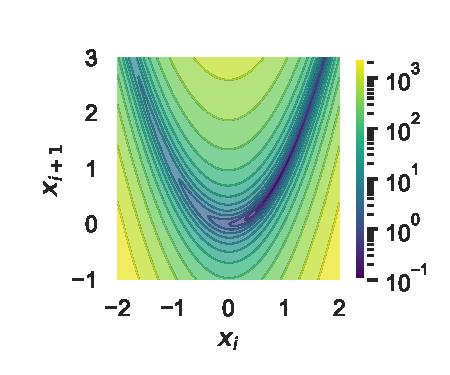
\includegraphics[width=4in]{../figures/rosenbrock_function.pdf}
    \caption{The Rosenbrock function, a classic optimization benchmark problem with mathematical formulation given in Equation \ref{eq:rosenbrock}. Here, the $N=2$ case is shown for ease of visualization, though axes are labeled as $x_i$ and $x_{i+1}$ to illustrate that this curving valley occurs in every adjacent pair of dimensions for higher-dimensional variants.}
    \label{fig:rosenbrock}
\end{figure}

\begin{figure}[h]
    \centering
    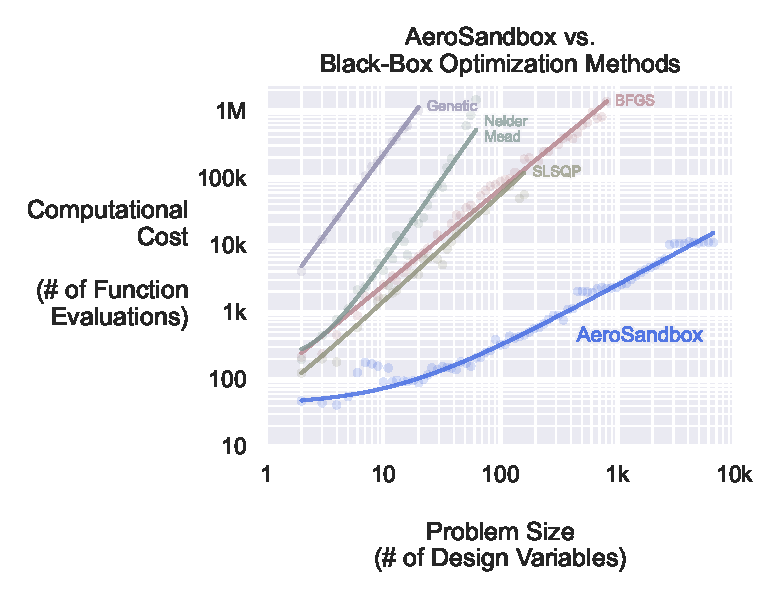
\includegraphics[width=\textwidth]{../figures/benchmark_nd_rosenbrock.pdf}
    \caption{Comparison of optimization performance between AeroSandbox and existing black-box optimization methods on the $N$-dimensional Rosenbrock problem. Other methods are two gradient-free methods (Nelder-Mead simplex method and a differential evolution genetic algorithm) and two gradient-based methods (SLSQP and BFGS), all using common SciPy implementations \cite{scipy}.}
    \label{fig:benchmark_nd_rosenbrock}
\end{figure}

In Figure \ref{fig:benchmark_nd_rosenbrock}, the computational cost of AeroSandbox (which leverages code transformations) is benchmarked against existing black-box optimization methods, as the problem dimensionality $N$ is varied. Several notable features can be seen in this figure. First, we find that gradient-based methods (e.g., BFGS, SLSQP) scale much better to high-dimensional optimization problems than gradient-free methods (e.g., Nelder-Mead, genetic), consistent with theory and other literature \cite{martins_engineering_2021, kochenderfer_algorithms_2019}. Because of this trend, these gradient-based methods are the most representative example of black-box methods used in industry today. As example points of comparison, the SUAVE aircraft design suite \cite{SUAVE2017} conventionally uses black-box SLSQP optimization, and the TASOPT aircraft design code \cite{drela_tasopt_2010} uses a black-box Nelder-Mead simplex method.

Second, we find that AeroSandbox offers significantly faster asymptotic runtime compared to all examined black-box methods. As problem dimensionality increases, the number of function evaluations required for AeroSandbox optimization to converge scales roughly linearly with the number of variables, while the equivalent metric for black-box gradient-based methods scales superlinearly. This improvement in scaling is mostly attributable to the use of automatic differentiation, which allows for more efficient gradient computation.

Third, we find that AeroSandbox offers improved convergence robustness to poor initial guesses compared to some methods, like SLSQP. In Figure \ref{fig:rosenbrock}, a method's convergence on the problem at a given dimensionality $N$ is shown by the presence or absence of a colored dot. While some methods converge fairly reliably (e.g., AeroSandbox and BFGS), others like SLSQP show more spotty convergence, with failure becoming increasingly common as the dimensionality increases. This is attributable to two factors: a) the backtracking line search implemented by IPOPT within AeroSandbox and the BFGS solver within SciPy, which stabilizes the optimization process, and b) the presence of automatic problem scaling, which improves the conditioning of the optimization problem.

A final possible contributor to differing performance may be gradient precision issues that can occur with black-box optimization, if such gradients are obtained by finite-differencing. In cases where this is severe, inaccuracies in gradient computation may result in slower optimization convergence in the black-box case. Generally, this is not an insurmountable issue, however, and Martins \cite{martins_engineering_2021} discusses possible options to mitigate this. For example, complex-step differentiation may be an option that enables higher precision if the black-box function handles (or can be modified to handle) complex data types with proper analytic continuation \cite{lai_extensions_2008, martins_complexstep_2003}.

In summary, this benchmark demonstrates that a code transformations paradigm can offer faster practical and asymptotic optimization performance than existing black-box optimization methods, especially as problem scale increases.

\subsection{Code Transformations vs. Disciplined Optimization Methods}
\label{sec:benchmark_gpkit}

Another MDO paradigm that can be compared to code transformation is a broad class of techniques known as disciplined optimization methods. The basic premise of such methods is that if user code can be restricted to specific mathematical forms, then specialized solvers can achieve large speedups over black-box methods. An example of one such mathematical form is convex optimization \cite{boyd_convex_2004}, and methodologies such as disciplined convex programming \cite{grant_disciplined_2006} show how a framework can be built on such paradigms. In these \emph{disciplined} frameworks, various mathematical properties (e.g., convexity) are tracked for each user-specified expression, to ensure that the optimization problem remains mathematically structured in a way that allows for a specialized solver.

From the perspective of aircraft design optimization, this paradigm became particularly intriguing with the advent of disciplined geometric programming \cite{boyd_tutorial_2007, agrawal_disciplined_2019}. In this method, we restrict not to the mathematical space of convex functions, but rather that of log-convex functions (i.e., monomials, posynomials, and signomials, which are described further by Burnell \cite{gpkit}). This interest from an engineering perspective is primarily due to research by Hoburg \cite{hoburg_geometric_2014}, who first applied such methods to conceptual aircraft design and demonstrated that many common first-order sizing relationships in this field are well-approximated by geometric programs. Further research by Hoburg, Kirschen, Ozturk, Burnell, and others \cite{kirschen, ozturk_conceptual_2018, jho} have extended this work with the development of GPkit, a geometric programming framework for engineering design optimization.

Using this framework, Kirschen shows that geometric programming (GP) methods can achieve significant runtime speedups over black-box optimization methods on engineering design problems \cite{kirschen}. In addition, this speedup is achieved largely without sacrificing the syntactical clarity of the user's code, which makes expressing design problems relatively efficient.

However, the mathematical restriction to certain categories of log-convex functions can be significant, and working around this by reformulation or approximation can sometimes prove burdensome in engineering practice. As an illustrative example, a case study by Vernacchia \cite{vernacchia_gpkit} documents an effort by an experienced end-user to build geometric-programming-compatible analysis tools for compressible aerodynamics. Here, a common empirical model for the transonic lift-curve slope ($C_{L\alpha}$) is found to break GP-compatibility due to the presence of a $\tan^2()$ function. To fix this, it is instead replaced with a modified \nth{12}-order Taylor series approximation. This strategy indeed works to restore GP-compatibility, but crafting such approximations can be both time-consuming and error-prone. These complex approximations can also lead to reduced interpretability during scenarios such as an engineering design review.

In some cases, approximation as a geometric program is not possible without unacceptable loss of fidelity, so models of interest must instead be written as \emph{signomial} programs \cite{ozturk_optimal_2021, kirschen}, a broader class of mathematical functions. This also works to restore compatibility with the framework, but sacrifices many of the benefits of geometric programming: most critically, problems become combinatorially-complex with respect to the number of signomial constraints. In both the case of geometric- and signomial-programming, these mathematical restrictions also limit the extensibility of design codes to higher-fidelity analyses, which are often not easily representable through such relationships.

Therefore, from this perspective, a valuable objective for any new MDO paradigm should be to achieve runtime speeds comparable to these disciplined optimization methods, while relaxing some of their mathematical restrictions to the extent possible. The code transformations paradigm that is proposed here achieves the latter goal of removing some mathematical restrictions: rather than restrict user code to log-convex expressions, the user is restricted to the much-broader category of $C^1$-continuous expressions. (Like disciplined methods, a specialized numerics library is still required, however. In the case of code transformations, this is due to the traceability requirement.) This relaxation of mathematical restrictions allows users to formulate many more engineering design problems without the need for mathematical rewriting, and the ability to embed common numerical operators such as linear solves and integrators enables extensibility to higher-fidelity modeling.

However, the question remains whether this relaxation of mathematical restrictions comes at the cost of computational performance. To investigate this, we conduct a benchmark study comparing code transformations (via AeroSandbox) to disciplined methods (via GPkit) on an example engineering problem. The specific problem is directly reproduced from the GPkit user documentation \cite{gpkit, gpkit_beam}, in order to ensure that a high-quality and representative GPkit code implementation is available for comparison. This problem in question is a static Euler-Bernoulli cantilever beam analysis problem, where a distributed load is applied; a diagram of the setup is shown in Figure \ref{fig:gpkit-cantilever-beam}. Values of various constants are taken from Burnell \cite{gpkit_beam} and reproduced in Listing \ref{lst:gpkit_beam}.

\begin{figure}[h]
    \centering
    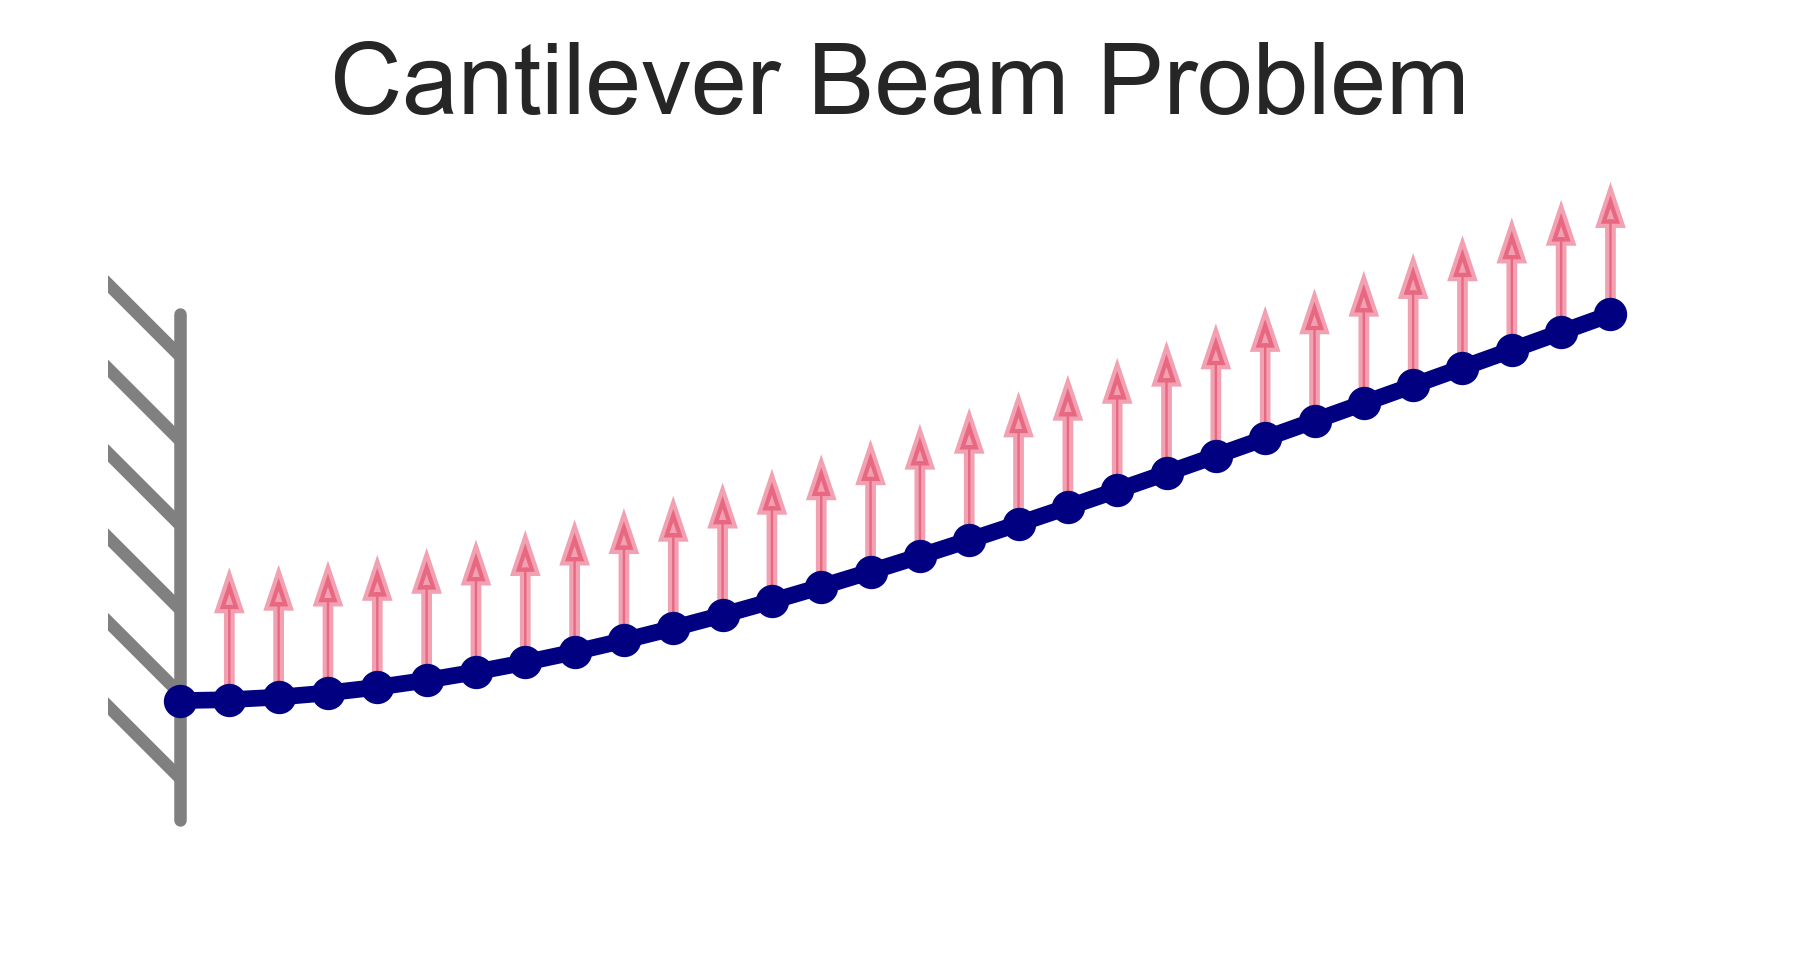
\includegraphics[width=3in,clip,trim={0 4.5cm 0 6.5cm}]{../figures/gpkit-compare/cantilever-beam.png}
    \caption{Setup for a cantilever beam analysis problem, which is identical to an example in the GPkit user documentation \cite{gpkit, gpkit_beam} and used as a benchmark to compare solution performance across various frameworks. The beam is discretized into $N$ elements, and a uniform distributed load is applied.}
    \label{fig:gpkit-cantilever-beam}
\end{figure}

Mathematically, this problem is represented as a fourth-order differential equation, which is discretized into $N$ elements. The goal of the analysis is to compute the state vector (deflection, slope, moment, and shear) at each point along the beam, given some specified distributed load. A useful observation is that, assuming the discretization is performed in a way that expresses integrands as a linear function of these state vectors (e.g., trapezoidal integration), this problem can be solved in a single sparse linear solve. However, this linearity is only advantageous if a framework can exploit this structure, and log-transformation will lose this property.

Numerically, the problem is written in residual (implicit) form, which allows it to be formulated as an optimization problem in various frameworks. As-given, this problem is a pure analysis problem, and the number of constraints (including boundary conditions) exactly equals the number of degrees of freedom. However, one can easily imagine this problem being implemented as a discipline-specific analysis within a larger MDO framework, where the beam analysis is coupled to other analyses (e.g., a wing sizing analysis) and design variables (e.g., wing thickness).

In Figure \ref{fig:benchmark_gp_beam}, the wall-clock runtime of AeroSandbox and GPkit is compared as the number of elements $N$ is varied. In this chart, four labeled cases are given:
\begin{enumerate}
    \item \textbf{GPkit (cvxopt)}, where the problem is solved using GPkit's default convex optimization solver, CVXOPT \cite{cvxopt}. Notably, CVXOPT is free and open-source, so the inclusion of this case allows an accurate ``open-source to open-source'' comparison to be drawn. The exact syntax used in this case (and in the MOSEK case below) is given by Burnell \cite{gpkit_beam}.
    \item \textbf{GPkit (mosek)}, where the problem is solved using GPkit's interface to a commercial solver, MOSEK \cite{mosek}. This is included to show the performance of GPkit in cases where users have access to a high-performance proprietary solver, and indeed the runtime is roughly an order of magnitude faster than the CVXOPT case.
    \item \textbf{AeroSandbox}, where the problem is formulated with syntax as close to its basic mathematical form as possible. The exact syntax used here is given in Listing \ref{lst:gpkit_beam}; notably, the coding style is declarative and allows the framework to set up its own discretization routines. In this case, a substantial speedup is achieved, in large part due to the fact that the problem is not solved in log-space, and hence the problem's natural linearity can be exploited by a gradient-based solver. Thus, in this case, the problem can always be solved in one optimization iteration.
    \item \textbf{AeroSandbox (using GP formulation)}, where the problem is given in its log-transformed form to AeroSandbox, which is identical to what underlying solvers of GPkit would see. This case is perhaps the most interesting of the four, because it shows that even with the same mathematical structure, code transformations can enable accelerations beyond what can be achieved with specialized solvers alone. In this case, subsequent benchmarking reveals that most of this additional speedup is due to sparsity detection and Jacobian compression, since the constraint Jacobian of this problem is quite sparse (due to locality of the governing equations).
\end{enumerate}

\begin{figure}[h]
    \centering
    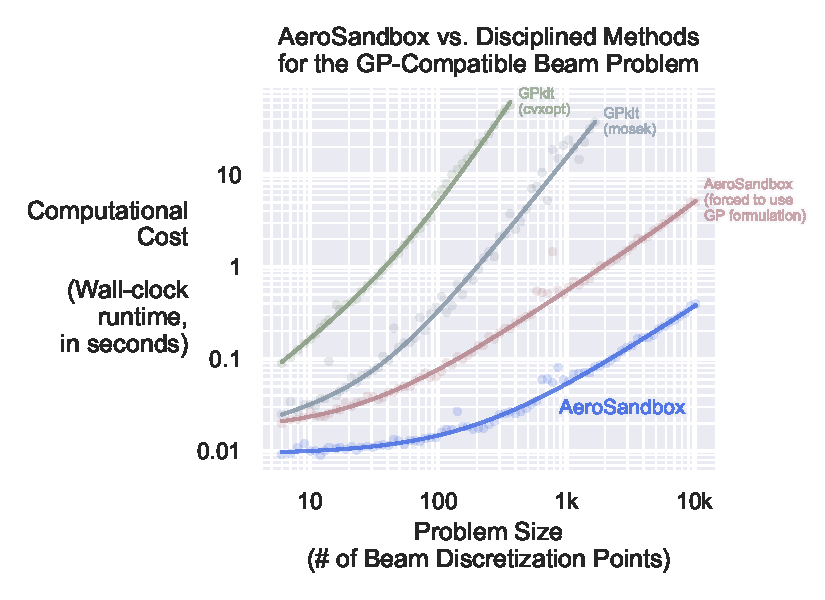
\includegraphics[width=\textwidth]{../figures/benchmark_gp_beam.pdf}
    \caption{Comparison of runtime speed between AeroSandbox and GPkit on the cantilever beam analysis problem. The problem is formulated as a static Euler-Bernoulli beam analysis, with the number of discretized elements, $N$, is varied to test scalability. The number of optimization variables (i.e., degrees of freedom) is $4N$, as the governing equation is originally a \nth{4}-order ODE and is decomposed to a larger system of first-order ODEs. In all cases, measured runtime includes both problem formulation and solution; time for library imports is excluded.}
    \label{fig:benchmark_gp_beam}
\end{figure}

Another interesting observation from Figure \ref{fig:benchmark_gp_beam} is the fact that the wall-clock runtime of the AeroSandbox case asymptotes to roughly 10 milliseconds in the limit of small $N$. This is rather large given the simplicity of the problem; if this analysis problem were explicitly formulated as a sparse linear program and given to such a specialized linear solver, it would likely be solved in a fraction of a millisecond. This discrepancy is due to the overhead of the optimization framework, which includes both tracing and applying code transformations. However, this overhead only scales weakly with problem size, and hence the runtime scales linearly with the number of elements $N$ in the limit of large $N$. This contrasts to the GPkit runtime, which scales superlinearly with $N$. This trend illustrates a common tradeoff in framework architectures: better asymptotic performance often comes at the cost of increased overhead for small problems, due to the need to find and exploit structure.

The payoff of this computational overhead, however, is that an end-user can take advantage of the sparse linear structure of the problem without needing to explicitly recognize and formulate it as such. This trades engineering effort for computational effort, which may be a favorable tradeoff in the context of quick-turnaround conceptual design problems. This automation also lowers the expertise barrier for users, as they do not need to be aware of the underlying mathematical structure of the problem to achieve good performance.

Other comparisons between a code transformations paradigm and disciplined optimization methods, including two conceptual aircraft sizing case studies, are given in prior work by Sharpe \cite{sharpe_aerosandbox_2021}. In short, code transformations can equal or exceed the runtime speed of disciplined optimization methods such as geometric programming, even on problems where this disciplined optimization approach is applicable. This is a promising result, as it suggests that code transformations may be able to offer the best of both worlds on engineering problems: the computational performance of disciplined optimization methods with fewer mathematical restrictions.

\subsection{Code Transformations vs. Analytic-Gradient Methods}

The final comparison to be made is between code transformations and an analytic-gradients paradigm, which focuses on using user-provided partial derivatives to facilitate gradient-based optimization. This is the preferred approach when especially fine-grained control over the MDO architecture and gradient computation process is required, as is often the case in high-fidelity engineering design optimization problems. The ability for users to directly patch in their own gradients is practically required to enable many advanced techniques in PDE-constrained optimization, such as adjoint methods and differentiable volume mesh morphing.

When implemented, user-specified analytic gradients can be faster than its code-transformations analogue of automatic differentiation. This is both for code reasons (e.g., the framework no longer incurs a tracing overhead) but also for mathematical ones (e.g., the ability to use continuous adjoints, for which there is no direct analogue in automatic differentiation \cite{rackauckas_universal_2021, rackauckas_direct_2022}).

However, the real benefit of analytic gradients is in the potential for reduced memory cost, especially in the case of the largest-scale design optimization problems. This is because the user can use strategies like checkpointing or time-reversal of ODEs to reduce the memory cost of gradient computation, which is challenging to automate in a general-purpose automatic differentiation framework \cite{chen2018neural, rackauckas_direct_2022, griewank_algorithm_2000}. For this memory reason, a framework based on analytic gradients is in fact the only tractable choice for many high-fidelity engineering design optimization problems.

Another framework benefit of ceding control over gradient calculation to user code is that it makes it cleaner to define disciplinary interfaces, as the ``components'' for which users specify partial derivatives form a natural disciplinary boundary. This can make it easier for the user to experiment with a wide variety of MDO architectures, which may improve performance in some cases \cite{martins_multidisciplinary_2013}. To contrast with this, the code transformations paradigm is more naturally suited to monolithic architectures (and in particular, simultaneous analysis and design) due to the global nature of the computational graph it constructs \cite{ma_modelingtoolkit_2021, haftka_simultaneous_1985}.

The primary downside of this analytic-gradients paradigm is that it requires substantial mathematical effort from the end-user. Formulating a quick design problem or extending existing analyses often requires hand-derivation and implementation of gradients, and this can stymie experimentation with radical design changes. In addition to the effort required, significant expertise in both mathematics and computer science is also required. Given that end users are often subject-matter-experts in their domain area, rather than in optimization \emph{per se}, this can restrict the potential user base. Even for experienced users, errors in user-specified gradients are a common and difficult-to-debug source of optimization failure.

Because of this, a code transformations paradigm may be a promising alternative to analytic-gradient methods in lower-fidelity design optimization cases, such as conceptual design. In such cases, where the fine-grained control of analytic gradients is less crucial, a simpler user experience that automates some of this optimization machinery may yield reduced overall user frictions. Because of this, Table \ref{tab:paradigm_comparison} suggests that the main advantage of a code transformations paradigm over analytic-gradient methods is improved ease of implementation.

To demonstrate what this looks like in practice, we implement a benchmark problem for comparison between AeroSandbox and OpenMDAO, which is a popular MDO framework that supports analytic gradients \cite{gray_openmdao_2019}. The specific problem is reproduced from the user documentation of OpenMDAO, once again to ensure that a high-quality implementation is available for comparison \cite{om_beam}. This problem is based on 1-dimensional Euler-Bernoulli beam theory, similar to the example of Section \ref{sec:benchmark_gpkit}. However, in this case it involves not just analysis but also optimization: the thickness of the beam along its length, $h(x)$, is a design variable. The beam is discretized into $N$ elements along its length, and the thickness distribution need not be uniform. A constraint on the total volume of the beam is imposed, and a cantilever boundary condition is applied. The optimization objective is to minimize the tip deflection of the beam while a point load is applied at the tip. This problem is illustrated in Figure \ref{fig:om-beam-opt}, with the actual optimal result of the beam design problem drawn to-scale\footnote{Although the assumed value for the bending stiffness $EI$ has been scaled for Figure \ref{fig:om-beam-opt} in order to make the deflection more visible.}. Additional numerical details and constants for this problem are available in Listing \ref{lst:om_beam}.

\begin{figure}[h]
    \centering
    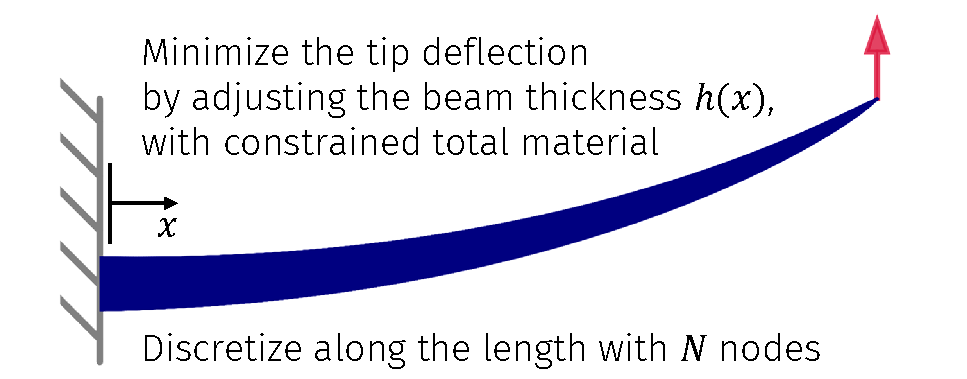
\includegraphics[width=4in]{../figures/om_beam-crop.pdf}
    \caption{High-level formulation of a beam shape optimization problem, which is identical to an example in the OpenMDAO user documentation \cite{gray_openmdao_2019, om_beam} and used as a benchmark to compare solution performance across various frameworks. The beam is discretized into $N$ elements along its length, with a point load at the tip.}
    \label{fig:om-beam-opt}
\end{figure}

In Figure \ref{fig:benchmark_om_beam}, we compare the wall-clock runtime of AeroSandbox and OpenMDAO as the number of beam discretization elements $N$ is varied. In the OpenMDAO case, the code implementation used for this comparison is given by the OpenMDAO development team \cite{om_beam}, and this implementation leverages exact analytic gradients. The corresponding code for the AeroSandbox case is given in Listing \ref{lst:om_beam}. In this benchmark study, we see that a code transformations framework can achieve faster runtime than analytic gradient methods across a range of discretization resolutions from $N=5$ to $N=500$.

\begin{figure}[h]
    \centering
    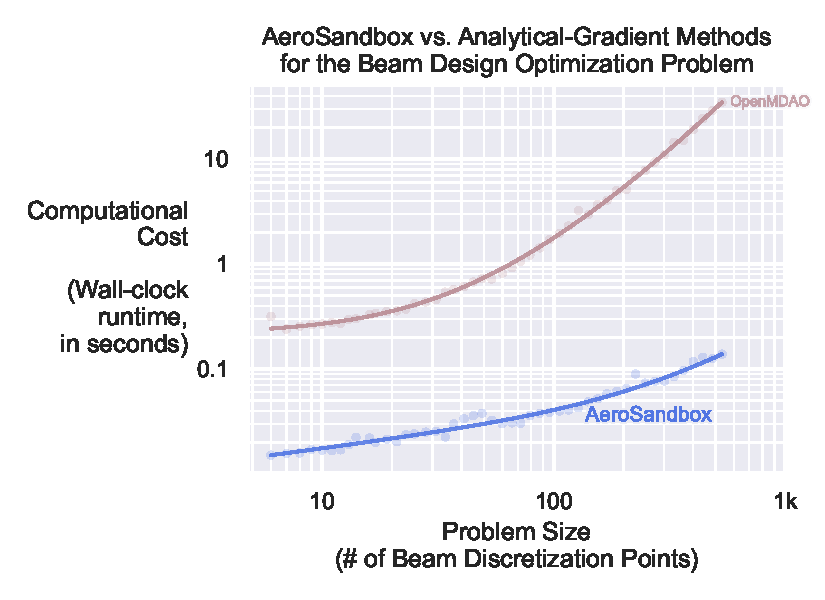
\includegraphics[width=\textwidth]{../figures/benchmark_om_beam.pdf}
    \caption{Comparison of runtime speed between AeroSandbox and OpenMDAO on the beam shape optimization benchmark problem. The number of discretized beam elements, $N$, varied to test scalability. In all cases, measured runtime includes both problem formulation and solution; time for library imports is excluded.}
    \label{fig:benchmark_om_beam}
\end{figure}

However, the true advantage of a code transformations framework in this case study is not in runtime speed, but rather in a reduction in engineering time. This ``code complexity'' is challenging to precisely quantify, but one possible (imperfect) metric for this is the number of user-written lines of code required to implement a given problem. Referencing the high-level overview of the optimization user experience in Figure \ref{fig:birds_eye_view}, this metric loosely corresponds to the amount of friction a user must overcome to implement a problem of interest. Table \ref{tab:benchmark_om_beam} shows that the AeroSandbox implementation of this problem requires roughly 8x fewer lines of code than the OpenMDAO one, which suggests that it requires much less engineering effort to develop.

\begin{table}
    \caption{Comparison of user-written lines of code and wall-clock runtimes between AeroSandbox and OpenMDAO on the beam shape optimization benchmark problem. AeroSandbox code implementation is available in Listing \ref{lst:om_beam}, and the OpenMDAO code implementation is given by the OpenMDAO development team \cite{om_beam}.}
    \label{tab:benchmark_om_beam}
    \begin{centering}
        \begin{tblr}{
            colspec={m{8cm} l l},
            row{1} = {font=\bfseries},
        }
            \toprule
            & AeroSandbox & OpenMDAO  \\ \midrule
            Problem-Specific Lines of Code$^\dagger$ & 35          & 287       \\
            Wall-Clock Runtime ($N=5$)               & 0.016 sec   & 0.253 sec \\
            Wall-Clock Runtime ($N=500$)             & 0.235 sec   & 31 sec    \\
            \bottomrule
        \end{tblr}
        \\
        \textcolor{darkgray}{$^\dagger$ Includes any imported utilities that are specifically pre-written for this beam problem.} \\
    \end{centering}
\end{table}

This discrepancy in engineering time occurs primarily because a true analytic-gradients framework requires every computation to be accompanied by a user-specified partial derivative\footnote{OpenMDAO allows users to fall back on black-box finite-differenced gradients, which brings both the advantages and drawbacks discussed in Section \ref{sec:benchmark-black-box}.}. This is true even for very simple calculations, such as the bending moment of inertia computation ($I=b h^3 / 12$) in this beam optimization benchmark problem. Furthermore, because these gradients must be linked to their respective functions, each of these computations requires the user to define a new class data structure\footnote{In OpenMDAO nomenclature, this is referred to as a \emph{component}} to package this information; this also increases the verbosity of the modeling language.

Another reason for the increased verbosity of the analytic-gradients paradigm is that the user must manually-construct component Jacobians if they wish to take advantage of sparsity. (In the case of a beam structural shape optimization problem, exploiting sparsity is essentially mandatory to achieve acceptable speed.) In the case of the OpenMDAO implementation of this benchmark problem, roughly half of the problem-specific lines of code are dedicated to assembling the beam's sparse stiffness matrix\footnote{In this code, definition of the per-element stiffness matrix takes 34 lines, and assembling these into a global stiffness matrix takes 113 lines. In total, the code is 287 lines.}. Furthermore, because assembly of the global stiffness matrix is performed on the user side of the interface, it is most naturally expressed via a loop in the same language facing the user: Python. This becomes a natural computational bottleneck as problem scale increases, which may induce the user to offload this to a different programming language, adding more complexity to the design tool. In contrast, a code transformations framework with both automatic differentiation and automatic sparsity detection capabilities can handle this task automatically. This sparsity detection can also occur in the language where the computational graph is represented (in the case of AeroSandbox's CasADi backend, C++), which can result in a substantial speedup.

For high-fidelity design optimization problems and for problems with only a handful of individual disciplines, shifting the responsibility of these numerical implementation details to the user may not be prohibitive; indeed, it may be necessary in cases. However, for conceptual design problems, which typically involve a vast number of low-fidelity models, and where the goal is to quickly explore a large configuration space, the engineering effort required here can be a significant barrier to entry.

\begin{listing}[h]
    \begin{minted}{python}
import aerosandbox as asb
import aerosandbox.numpy as np

N = 500  # Number of discretization nodes
E = 1e3  # Elastic modulus [N/m^2]
L = 1  # Beam length [m]
b = 0.1  # Beam width [m]
volume = 0.01  # Total material allowed [m^3]
tip_load = 1  # Tip load [N]

x = np.linspace(0, L, N)  # Node locations along beam length [m]

opti = asb.Opti()  # Initialize an optimization environment
h = opti.variable(init_guess=np.ones(N), lower_bound=1e-6)  # Beam thickness [m]
I = (1 / 12) * b * h ** 3  # Bending moment of inertia [m^4]

V = np.ones(N) * (-tip_load)  # Shear force [N]
M = opti.variable(init_guess=np.zeros(N))  # Moment [N*m]
th = opti.variable(init_guess=np.zeros(N))  # Slope [rad]
w = opti.variable(init_guess=np.zeros(N))  # Displacement [m]

opti.subject_to([  # Governing equations
    np.diff(M) == np.trapz(V) * np.diff(x),
    np.diff(th) == np.trapz(M / (E * I), modify_endpoints=True) * np.diff(x),
    np.diff(w) == np.trapz(th) * np.diff(x),
])
opti.subject_to([  # Boundary conditions
    M[-1] == 0,
    th[0] == 0,
    w[0] == 0,
])
opti.subject_to(np.mean(h * b) <= volume / L)  # Volume constraint
opti.minimize(w[-1])  # Objective: minimize tip deflection
sol = opti.solve()
print(sol(h))  # Gives the optimized beam thickness
    \end{minted}
    \caption{AeroSandbox implementation of the beam shape optimization problem. Written in Python.}
    \label{lst:om_beam}
\end{listing}

It is important to emphasize that, although this study demonstrates some challenges of using a framework based on analytic-gradients for conceptual design purposes, doing so is absolutely possible. Several successful efforts such as the OpenMDAO-based OpenConcept \cite{Brelje2018a} and its related OpenAeroStruct \cite{Adler2022d} provide existence proofs of this; the code architectures of these tools provide useful examples of how conceptual design workflows within this paradigm can be structured. In these cases, the user experience is streamlined by a framework-provided library of pre-written components that encapsulate common disciplinary analyses, each of which also has manually-implemented analytic gradients. This can be a suitable approach, especially in targeted applications where the user's design intent does not deviate too far from the assumptions of these pre-written analyses. However, the end-user experience becomes substantially more challenging when the user needs to extend these analyses or pose design problems outside the intended application scope of the framework, as they are no longer insulated from the frictions outlined here.

Because of these reasons, we generally assess that a code transformations paradigm offers improved ease of implementation compared to analytic-gradient methods, as depicted in Table \ref{tab:paradigm_comparison}. This is especially true for conceptual design problems, where the user's primary goal is to quickly explore a large configuration space. Of course, for high-fidelity design optimization problems, where very fine-grained control over numerical processes is required, an analytic-gradients paradigm likely remains more suitable.

In all three of the comparison case studies examined in this section, it becomes clear that most framework architecture decisions ultimately come down to tradeoffs: usability, runtime speed, and mathematical restrictions must all be considered. The best choice of MDO paradigm for a given design problem will depend on the specific requirements of that problem, and the user's expertise and preferences. However, the results of these benchmark studies suggest that a code transformations paradigm can offer a favorable general-purpose compromise between these factors, especially in the context of conceptual design optimization problems.


\section{Syntax and Interface Considerations}
\label{sec:syntax-interface}

The benchmark studies of Section \ref{sec:benchmarks} discuss a variety of considerations to be weighed when developing an engineering design optimization framework, and how different architectural choices link to these tradeoffs. From these studies, we can begin to extract a more concise list of the high-level opportunities and challenges of using a code transformations paradigm for engineering design optimization, relative to other options:

\begin{itemize}
    \item \textbf{Opportunities} (in the context of conceptual-level engineering design optimization):
    \begin{enumerate}
        \item Code transformations yield performance comparable to bespoke, efficient numerical code, while reducing the amount of problem-specific code that users must write. Although there are many cases where performance could be further accelerated with more specialized numerics, we contend that code transformations generally represent a useful ``80/20'' Pareto tradeoff for the end user: they achieve most of the performance of bespoke code with a fraction of the engineering effort.
        \item By adding more separation between the problem formulation (i.e., physics modeling) and the numerical optimization process, code transformations let engineers focus on asking the right design question. As noted by Drela \cite{drela_pros_1998}, developing a problem formulation that faithfully represents design intent is often the most challenging part of practical engineering design optimization. By abstracting away some elements of the numerical optimization process by default, code transformations can help users focus on this critical aspect of the design process.
    \end{enumerate}
    \item \textbf{Challenges}:
    \begin{enumerate}
        \item As alluded to in Section \ref{sec:traceability}, the requirement that user-written numerical code be traceable imposes some restrictions on the end-user; the severity of this falls somewhere between that of the black-box- and disciplined-optimization paradigms. Most fundamentally, the user must formulate their design problem using syntax from a framework-provided numerics library, to allow tracing. This naturally creates a tension against usability, and choices about the syntax of this specialized numerical library can strongly affect the learning curve of an MDO framework.
        \item Beyond just the \emph{syntax} of a user's numerical code, a code transformations paradigm also imposes certain preferences on the \emph{style} of a user's numerical code. In particular, for reasons discussed in Section \ref{sec:code_style}, this paradigm favors a \emph{functional} coding style that avoids side effects and mutable state, since this is more easily traced and transformed. In contrast to this, we later argue that the workflow of engineers working on physics-based design optimization problems naturally tends to lead to \emph{procedural} coding styles, which creates another source of tension in framework development.
    \end{enumerate}
\end{itemize}

It is worth noting that both of the listed challenges of code transformations relate to framework-level tensions between the user experience and computational performance. This motivates a renewed focus on framework choices around syntax and interfaces, since these play a key role in determining the practicality of an MDO framework.

\subsection{Implications of Code Transformations on Coding Syntax}
\label{sec:code_syntax}

The main requirement for code transformations, traceability, requires user code to be built on top of a custom numerics library. To minimize the syntax burden associated with this library, one possible strategy is to design the library to closely resemble the syntax of an existing common numerical computing library, such as NumPy \cite{harris_array_2020}. In fact, one can even implement a direct 1:1 drop-in replacement for this numerical library, which enormously reduces the learning curve for the end user. The first major successful application of this strategy was with the advent of Autograd, an automatic differentiation library by Maclaurin et al. \cite{maclaurin_autograd_2015}.

Inspired by this, AeroSandbox takes a similar approach of mirroring a NumPy-like interface for numerical operations, but with the added capability of tracing code execution. Access to this interface is enabled by essentially hijacking the user's NumPy import, which commonly occurs at the beginning of a user-specified analysis; this is shown in Figure \ref{fig:asb-np-import}. Because many engineers already write analysis code with NumPy syntax, writing new code and migrating existing analyses becomes much easier -- in many cases, the only required change is a single import statement.

\begin{figure}[H]
    \centering
    \begin{tikzpicture}[
    auto,
    node distance=3cm
]
    \tikzstyle{code} = [
    draw = c1, fill = c1!20,
    minimum height = 1cm,
    rectangle, rounded corners, thick,
%    text width = 7cm,
    text centered,
    ]

    \tikzstyle{line} = [thick, ->, shorten >=2pt, shorten <=2pt]

    \node[code](np) {\mintinline{python}{import numpy as np}};
    \node[code, right=of np](asb) {\mintinline{python}{import aerosandbox.numpy as np}};

    \draw [line](np) -- (asb) node [midway, above, sloped](text){becomes};

\end{tikzpicture}
    \caption{Standard import of the AeroSandbox numerics stack, which acts as a drop-in replacement for the user's NumPy code. Figure reproduced from Sharpe \cite{sharpe_aerosandbox_2021}.}
    \label{fig:asb-np-import}
\end{figure}

In recent years, there has been growing momentum in the Python scientific computing community to develop a unified ``array API'' standard, to greatly expand interoperability and extensibility of numerical libraries \cite{array_api_2023}. This standard, which is being jointly developed by a consortium of developers representing various popular numerics libraries\footnote{such as NumPy, PyTorch, Tensorflow, JAX, and others}, aims to provide a common interface for numerical operations that can be implemented by any array library. If this standardization effort is successful, it may be possible within the next few years to hook into numerical function calls without replacing the imported library, making the end-user experience even more seamless.

When implementing a specialized array library such as the one illustrated in Figure \ref{fig:asb-np-import}, each function must be overwritten to allow for tracing. This can place a substantial burden on the framework developer, both in the initial development phase but also in terms of ongoing maintenance as the syntax of the mirrored library changes. Because of this, selecting the appropriate ``attack surface'' of numerical functions is crucial: too small, and the user's ability to express their design problem is limited; too large, and the framework developer is overwhelmed with maintenance tasks. To balance these competing tradeoffs, the AeroSandbox numerics library aims to recreate a carefully-chosen subset of commonly-used NumPy and SciPy functions, including:

\begin{itemize}[noitemsep]
    \item Array operations (initialization, indexing, concatenation, stacking, reshaping, etc.)
    \item Elementary functions (arithmetic, trigonometry, special functions, etc.)
    \item Conditionals and boolean logic\footnote{A particularly useful inclusion is the NumPy \texttt{where()} function, which allows element-wise conditional assignment. Note that the framework does not explicitly enforce $C^1$-continuity of the user's code across conditional boundaries, but attempting to optimize while using $C^1$-discontinous functions will often cause convergence issues. Further discussion is given in prior work by Sharpe \cite{sharpe_aerosandbox_2021}.}
    \item Linear algebra
    \begin{itemize}[noitemsep]
        \item Einstein-summation operations (matrix products, dot products, outer products, etc.)
        \item Vector and matrix norms
        \item Linear solves, Moore-Penrose pseudoinverses
        \item Various factorizations (e.g., eigenvalue decomposition)
    \end{itemize}
    \item Various common utility functions (e.g., \texttt{linspace()})
    \item Interpolation, including N-dimensional and higher-order variants, and both gridded and scattered methods
    \item Higher-order discrete numerical differentiation (i.e., gradient reconstruction, for ODEs and PDEs)
    \item Higher-order numerical integration and quadrature, in both continuous and discrete variants (e.g., acting on either functions or sampled data)
    \item Coordinate transformations and rotations
    \item Surrogate modeling and regression tools (e.g., curve fitting tools, kriging, neural network activation functions, orthogonal polynomial families, etc.)
\end{itemize}

In the author's experience, this subset of functions is sufficient to express a wide variety of engineering design problems, and is a good starting point for a general-purpose engineering design optimization framework. However, the exact choice of functions to include will depend on the specific application domain of the framework.

The author's prior Master's thesis \cite{sharpe_aerosandbox_2021} further discusses these syntax-related choices and tradeoffs that should be considered when developing an MDO framework, using examples from the development of AeroSandbox.

\subsection{Implications of Code Transformations on Coding Style}
\label{sec:code_style}

Another relevant consideration in the development of a numerical framework that allows for code transformations is the coding style that is encouraged by the paradigm. In particular, it is much easier to write a traceable numerics stack if one can guarantee that the user's code follows a \emph{functional} programming style, which avoids side effects and mutable state (collectively called ``in-place operations'', since they modify an array without allocating a new memory register). This is because it the most natural way to store intermediate values of a computational graph during evaluation is by directly attaching them to graph nodes. If code is mutable, then different nodes in the graph may point to the same array -- in other words, the same memory location. (An example of this is a pair of nodes that occur immediately before and after an indexed array assignment). This leads to a overwriting of intermediate values during execution. Unfortunately, many code transformations rely on accessing these intermediate values -- for example, reverse-mode automatic differentiation requires these values to evaluate the backward pass.

To address this, some early numerics libraries that support dynamic tracing, like Autograd \cite{maclaurin_autograd_2015, maclaurin_modeling_2016}, simply forbid mutable state in user code -- a functional programming style is required. PyTorch takes a similar approach, though a bit less severe: instead, the developers heavily discourage in-place operations, though still makes an attempt to handle them by attaching a ``version counter'' to each array that is incremented upon mutation \cite{paszke_pytorch_2019}. This approach does not work in a fair number of cases\footnote{An example of this is when the array is externally-referenced both before and after mutation, since this makes memory duplication unavoidable and requires a computational graph rewrite}, but it allows PyTorch to support limited mutation in user code. Critically, in cases where this is not possible, the counter system allows PyTorch to alert the user, rather than silently producing incorrect results.

On the other hand, other tracing-compatible numerics libraries make an attempt to work around this limitation syntactically, which can allow the use of other coding styles (to varying degrees). For example, while JAX \cite{jax} does not directly support in-place operations, it does offer the user alternative syntax that can be used to replace in-place array element assignments with functional-style array transformations\footnote{For example, in JAX, the in-place code \mintinline{python}{x[0] = 5} can be roughly replaced by the functional code \mintinline{python}{x_new = x.at[0].set(5)}. This places some burden of understanding mutability on the end-user, but in most cases it at least allows some workaround to be performed here.}.

The CasADi numerics library implements an particularly sophisticated approach that completely allows for in-place mutation; to the best of the author's knowledge, this is the only Python-based automatic differentiation library\footnote{among those that support both forward- and reverse-mode automatic differentiation} that achieves this. This is done by completely decoupling the tracing and evaluation of the computational graph, with two independent ``register-based virtual machines'' that separately store the traced graph and the executed graph. As described by Andersson et al. \cite{andersson_casadi_2019}:

\begin{quote}
    ``The creation of [an executable expression] in CasADi essentially amounts to topological sorting the expression graph, turning the directed acyclic graph (DAG) into an \emph{algorithm} that can be evaluated. Unlike traditional tools for AD\ldots, there is no relation between the order in which expressions were created (i.e., a \emph{tracing step}) and the order in which they appear in the sorted algorithm.''
\end{quote}

\noindent This solves the problem of intermediate value preservation at its root, since during evaluation, these numerical values are no longer directly attached to graph nodes, but instead stored in a separate memory register (possibly, with different graph topology than the initial computational graph). To the end user, the net result is that they can write code in a procedural style, with in-place operations, and still have it be traced and differentiated. This is one of the main reasons why AeroSandbox makes the framework-level design decision to default to a CasADi-based numerical backend: it gives the user flexibility to write mutating code.

\subsubsection{Coding Styles and the Engineering Design Workflow}

We contend that lifting this restriction on only using functional coding styles offers significant usability advantages for engineering design applications. This stems from a belief that the natural workflow of engineers often leads to \emph{procedural} coding styles, where the bulk of the logic is expressed as a sequence of (possibly stateful) instructions, rather than within the stricter confines of pure functions. To put it more colloquially, engineers tend to write their analyses into things that look more like scripts or spreadsheets, and less like libraries. To illustrate why this procedural coding style is popular in engineering practice, consider a representative hypothetical example of how an industry engineer might arrive at the decision to use a design optimization framework:

\begin{enumerate}
    \item When an engineer initially embarks on a new development effort, the first computational task that an engineer will usually perform is a quick back-of-the-envelope forward analysis to develop some intuition: ``Assuming some reasonable design, what information do I need to make a reasonable estimate about its performance?'' This is usually done as a simple procedural script or spreadsheet, and the goal is not to optimize the design but rather to start understanding the problem physics and design drivers.

    For example, suppose an engineer wants to perform basic wing sizing. Often, the first attempt at this problem will be to simply implement a forward analysis: assume a representative wing, and estimate its lift and drag using basic aerodynamic theory. The assumed wing might look something like Figure \ref{fig:proc_wing}. In code, this might look like Listing \ref{lst:proc_wing}.

    \begin{figure}[H]
        \centering
        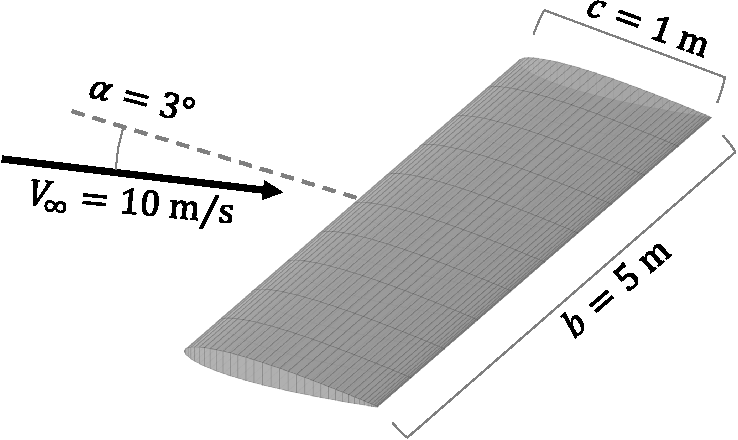
\includegraphics[width=4in]{../figures/wing_proc-crop.pdf}
        \caption{An example of an initially-assumed problem geometry for a wing sizing analysis.}
        \label{fig:proc_wing}
    \end{figure}

    \begin{listing}[H]
        \begin{minted}{python}
import numpy as np

kinematic_viscosity = 1.461e-5  # air, at 20 C [m^2/s]
airspeed = 10  # [m/s]
alpha = 3 # Angle of attack [deg]
chord = 1  # [m]
span = 5  # [m]

CL = (2 * np.pi) * np.radians(alpha)  # Lift coeff., based on thin airfoil theory

Re = airspeed * chord / kinematic_viscosity  # Reynolds number [-]
CD_p = 1.328 / np.sqrt(Re)  # Profile drag coeff., based on Blasius BL

AR = span / chord  # Aspect ratio [-]
CD_i = CL ** 2 / (np.pi * AR)  # Induced drag coeff., based on theory

CD = CD_p + CD_i  # Total drag coefficient

print(CL / CD)  # Result: 38.7
        \end{minted}
        \caption{Example of a simple forward analysis script to estimate the aerodynamic performance of an untapered, unswept, untwisted, planar wing using napkin-math-level theory.}
        \label{lst:proc_wing}
    \end{listing}

    \item So far, one could argue that the code in Listing \ref{lst:proc_wing} could be considered both procedural and functional, because despite the single-level scope of the analysis, it is stateless and non-mutating. However, consider what happens when the engineer wants to build on top of this analysis and start asking natural next-step questions. For example, ``What is the minimum-drag wing that is possible, if the geometry and angle of attack are varied?'', and ``How does the resulting design need to change if an implicit lift-weight closure is enforced, with some assumed wing weight model?''

    In frameworks that require a functional style, we would need to rewrite the script with several major changes. First, the problem would need to be structured as a single top-level function wrapper that takes in all variables and returns all constraints and the objective\footnote{A code example of this, for the curious reader, is in the publically-available FBHALE MDO code. Here, a single top-level master function takes in all variables and returns all constraints.}. Secondly, as a practical matter, all disciplinary analyses would need to be rewritten as standalone pure functions. (This makes little difference in this simple example, but in more complex MDO problems with hundreds of interacting models, this creates an enormous amount of boilerplate code and obfuscates design intent.) An undesirable side effect of all of this added boilerplate code is that it ``locks in'' the problem formulation -- changing what is a variable and what is a constraint requires a substantial rewrite of the entire analysis.

    Within frameworks that allow optimization formulation in a procedural style, however, converting this initial analysis into a design problem becomes far easier. Expressing this optimization problem becomes a natural extension of the initial analysis, and this can be achieved \emph{without adding new scopes}.

    To show this more concretely, Listing \ref{lst:proc_wing_opt} gives an example of how a user might extend the initial analysis from Listing \ref{lst:proc_wing} to a simple design optimization problem that answers these questions. This listing uses syntax from AeroSandbox, a design optimization framework that supports procedural coding styles. In Listing \ref{lst:proc_wing_opt}, the lines of code that differ from the original code of Listing \ref{lst:proc_wing} are highlighted, which shows the minimal change in overall code structure. Notably, new variables and constraints are simply ``tagged'' during the problem specification, rather than requiring a functional-style rewrite of the entire analysis. Even an implicit constraint (the lift-weight closure) can be expressed in a single line of code, without pulling out the evaluation of this constraint into a separate function.

    \begin{listing}[H]
        \begin{minted}[highlightlines={1-2,4,9,11-12,24-26,28-29}]{python}
import aerosandbox as asb
import aerosandbox.numpy as np  # Patches in the AeroSandbox numerics stack

opti = asb.Opti()  # Start an optimization environment

kinematic_viscosity = 1.461e-5  # at 20 C [m^2/s]

airspeed = 10  # [m/s]
alpha = opti.variable(init_guess=3) # Angle of attack [deg]

chord = opti.variable(init_guess=1, lower_bound=0)  # [m]
span = opti.variable(init_guess=5, lower_bound=0)  # [m]

CL = (2 * np.pi) * np.radians(alpha)  # Lift coeff., based on thin airfoil theory

Re = airspeed * chord / kinematic_viscosity  # Reynolds number [-]
CD_p = 1.328 / np.sqrt(Re)  # Profile drag coeff., based on Blasius BL

AR = span / chord  # Aspect ratio [-]
CD_i = CL ** 2 / (np.pi * AR)  # Induced drag coeff., based on theory

CD = CD_p + CD_i  # Total drag coefficient

lift = 0.5 * 1.225 * airspeed ** 2 * CL * chord * span  # Lift force [N]
weight = (1 + chord * span ** 2) * 9.81  # A simple hypothetical weight model [N]
opti.subject_to(lift == weight)  # Implicit L=W constraint

opti.minimize(CD)  # Objective function
sol = opti.solve()  # Solves the problem

print(sol(CL / CD))  # Result: 115.2
        \end{minted}
        \caption{Example of a simple design optimization problem to find the minimum-drag wing, starting from the initial analysis in Listing \ref{lst:proc_wing}. Highlighted lines show elements added or modified from the initial analysis.}
        \label{lst:proc_wing_opt}
    \end{listing}

    The ability to support these inline definitions of optimization problem elements makes it much easier to rapidly ``turn the problem around'' and change the problem formulation between the forward problem (analysis) and the inverse problem (optimization). For example, changing the problem parameterization (i.e., which variables is the optimizer free to modify, and which are frozen to assumed constants) typically requires significant rewriting in a functional problem formulation, but in a procedural one this becomes a seamless one-line code change. This becomes especially apparent in large-scale MDO problems, where restricting the user to a functional coding style forces them to be much more careful with sequencing the analysis order to maximize feed-forward information flow\footnote{because functional coding forces much more partitioning into separate scopes, and required information needs to be ``piped around'' to the appropriate scope level}.

\end{enumerate}

Based on this example, we contend that optimization applications to engineering design benefit strongly from a framework that allows for a procedural coding style -- this tends to naturally mimic the workflow of practicing engineers as they incrementally develop their problem from analysis into optimization. An interesting observation is that this contrasts against the needs of other applications of traceable numerics frameworks, like machine learning. For example, Autograd developer Maclaurin \cite{maclaurin_modeling_2016} states that ``Our experience using Autograd has been that a functional style is a natural fit for the sorts of modeling and inference problems we like to solve in machine learning, and it rarely feels burdensome.'' This makes sense, because machine learning workflows tend to involve relatively simple expressions that are data-heavy but operator-light\footnote{Consider that a multi-layer perceptron may consist of millions of parameters, but the forward pass can still be expressed in a dozen or so large kernel operators in code. By contrast, an engineering MDO tool may have hundreds of empirical curve-fit-style models, leading to much more complex computational graphs and information flow.}, while engineering workflows tend to use expressions that are data-light but operator-heavy. (This can be seen in the example engineering computational graph of Figure \ref{fig:computational-graph-aerosandbox}.) This highlights that, although engineering design optimization has benefited heavily from machine learning advances in the past decade, there are some fundamental reasons why tools developed for machine learning are often not perfectly suited for direct use in engineering design optimization, and therefore frameworks designed with this purpose in mind are advantageous \cite{rackauckas_engineering_2021}.

\subsection{Miscellaneous Considerations}

A final relevant choice that any engineering design framework needs to consider is how to handle units in dimensional quantities, if at all. This is particularly interesting in the context of code transformations, because standard ways of handling units essentially ``box'' all dimensional quantities within a specialized data structure that contains both the numerical value and the associated unit\footnote{For example, see the Pint package in Python \cite{pint}, or Unitful.jl in Julia \cite{unitful}.}. Predictably, this can cause problems when tracing, since it forces expressions to use (and expect) specific data types -- the units container. Because of this, passing a dynamic tracer object through the user analysis may not be possible, as functions are no longer type-agnostic. Hence, adding a required units system to an MDO framework often fundamentally-precludes strategies that rely on code transformations.

Even if this traceability issue is fixed, boxing all quantities in units objects also incurs significant performance penalties -- regardless of whether code transformations are used. It is not uncommon to see order-of-magnitude slowdowns in engineering code that attempts to directly embed units. This is mostly due to two reasons. First, it forces functions to do type-checking and units propagation (essentially, a symbolic algebra step) on every operation, which is a significant overhead in operator-heavy code\footnote{An interesting analogy is that this is slow for the same reason that type-unstable numerical code (e.g., most Python code, where the heavy lifting is done in Python, like direct looping) is slower than type-stable code (e.g., code in any static language, like C++ or Fortran).}. Secondly, this units-container data structure forces numerical data to be stored on the memory heap, rather than the stack (where intermediate arrays would normally be stored), which is slower due to the increased memory access latency. This problem becomes even worse if the user wishes to perform any hardware acceleration (e.g., GPU computing) or , since the container must be packed and unpacked at each operation.

Because of these reasons, even though explicitly storing units in engineering analyses and MDO frameworks may initially seem attractive, it usually results in significant headaches down the line. Of course, it is still useful to have some strategy for preventing potentially-costly unit misunderstandings. Over the years, several strategies have emerged that, in the author's opinion, are superior to the direct unit-boxing approach:

One possible existing strategy is aggressive non-dimensionalization, where all user inputs and outputs are either expressed in nondimensional quantities, or (in cases where this is not possible) immediately nondimensionalized after input. This is a particularly common strategy in aerodynamics codes, as seen in codes like AVL \cite{avl}, SU2 \cite{economon_su2_2016}, Flow360, and others. However, while this strategy works well within a single tightly-scoped analysis, is not necessarily scalable for large multidisciplinary problems. In these large MDO codes, attempting to pass around a set of global reference quantities to all analyses quickly becomes unwieldy, so global nondimensionalization is not a practical solution.

An alternative strategy, and the one used by AeroSandbox, is simply to establish a convention that all variables are in base units from some globally-used \emph{coherent}\footnote{I.e., a system of units that involves no internal conversion factors; all derived units are products of powers of base units, with no scaling factors.} units system, or derived units thereof. The most obvious such coherent system is SI, but others (e.g., foot-pound-second, using slugs for mass) are also feasible. AeroSandbox assumes an SI system, and hence all variables are in base or derived quantities (e.g., m, kg, sec, N, m/s, J, Pa, etc.). Regardless of the system chosen, coherence allows all derived units to be implemented without any scaling factors or unit wrappers, which improves both readability and computational performance.

In this strategy, unit interpretation can be facilitated by clear, interpretable variable names that make the expected dimensions of a given quantity unambiguous to the user; in the age of autocomplete in modern code editors, this requires minimal effort. In cases where long-standing industry convention is to use non-coherent units, this can easily be handled by an explicit indicative suffix. For example:

\begin{itemize}[noitemsep]
    \item \mintinline{python}{battery_capacity} $\rightarrow$ Joules
    \item \mintinline{python}{battery_capacity_kilowatt_hours} $\rightarrow$ kilowatt-hours
    \item \mintinline{python}{aircraft_endurance} $\rightarrow$ seconds
    \item \mintinline{python}{aircraft_endurance_hours} $\rightarrow$ hours
\end{itemize}

A consequence of this strategy is that quantities may differ in numerical value by many orders of magnitude; an elastic modulus may be on the order of $10^{11}$ Pa, while a wing skin thickness may be on the order of $10^{-3}$ m. Many years ago, when single-precision floating-point arithmetic was the norm, this could cause numerical issues due to the limited dynamic range of the data type. However, with the advent of double-precision floating-point arithmetic as the standard, this is nearly never an issue in practice. One could also be reasonably concerned that this scaling difference could cause optimization difficulties\footnote{because, although most second-order gradient-based optimziation algorithms are mathematically scale-invariant, the poor condition number of the Hessian (or Hessian approximation) could make for inaccurate steps}; however, with the automatic scaling performed with AeroSandbox, all quantities are brought to a similar order of magnitude before the problem is passed to the optimizer, and this is not an issue.

Because of these considerations, the author recommends that code-transformation-based MDO frameworks avoid explicitly embedding units in the code via unit-boxing strategies, and instead rely on a coherent units system and clear variable naming conventions to prevent unit misunderstandings. This strategy is both more performant and more flexible, and industrial users of AeroSandbox have generally reported that this approach is intuitive and easy to adopt.


\section{Computational Reproducibility}
\label{sec:asb-reproducibility}

Source code, installation instructions, documentation, and walkthrough tutorials for the AeroSandbox framework are available at \url{https://github.com/peterdsharpe/AeroSandbox}. All materials are released under the MIT License, which allows broad permissions on how the software can be used.

The framework is also available on the Python Package Index (PyPI) as the package \texttt{aerosandbox}; to install, use the command \texttt{pip install aerosandbox[full]}, where the \texttt{[full]} suffix causes optional dependencies to be installed as well. For users less familiar with the Python packaging ecosystem, a step-by-step walkthrough of the installation process can be found in the appendix of prior work by Sharpe \cite{sharpe_aerosandbox_2021}.